\section{Games with imperfect information}

Sometimes players must make moves at the same time, and so they cannot have full knowledge of each other’s moves. 
This can be still represented with a tree.
\begin{figure}[H]
    \centering
    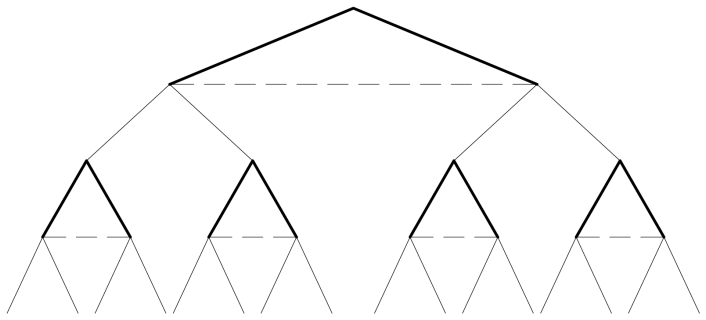
\includegraphics[width=0.75\linewidth]{images/tree3.png}
    \caption{Tree with imperfect information}
\end{figure}
Dashed line: the player does not know exactly which vertex she finds herself in.

\begin{definition}[\textit{Information set}]
    An information set for a player $i$ is a pair $(U_i, A(U_i))$ with the following properties:
    \begin{enumerate}
        \item $U_i \subset P_i$ is a nonempty set of vertices $v_1, \cdots, v_k$
        \item each $v_j\in U_i$ has the same number of childre. 
        \item $A_i(U_i)$ is a partition of the children of $v_1 \cup \dots \cup v_k$ with the property that each element of the partition contains exactly one child of each vertex $v_j$
    \end{enumerate}
\end{definition}
Accordingly, player $i$ knows to be in $U_i$, but not in which vertex she is.
The partition yields the choice function, meaning that each set in $A_i(U_i)$ represents an available move for the player (graphically, it is the same choice, i.e. an edge, coming out of the different vertices).
\begin{definition}[\textit{Extensive form game with imperfect information}]
    An Extensive form Game with imperfect information is constituted by: 
    \begin{enumerate}
        \item A finite set $N = \{1, \dots, n\}$ of players. 
        \item A game tree $(V, E, x_0)$. 
        \item A partition made by sets $P_1, P_2, \dots, P_{n+1}$ of the vertices which are not leaves.
        \item A partition $(U^j_i), j = 1, \dots, ki$ of the set $P_i$, for all $i$, with $(U^j_i, A^j_i)$ information set for all players $i$ for all vertices $j$ (with the same number of children). 
        \item A probability distribution, for each vertex in $P_{n+1}$, defined on the edges going from the vertex to its children. 
        \item An $n$-dimensional vector attached to each leaf
    \end{enumerate}
\end{definition}
Note that if the partition comprises just a single vertex, then a game with imperfect information becomes the same as a game with perfect information.
\begin{definition}[\textit{Pure strategy}]
    A pure strategy for player $i$ in an imperfect information game is a function defined on the collection $\mathcal{U}$ of his information sets and assigning to each $U_i$ in $\mathcal{U}$ an element of the partition $A(U_i)$. 
    A mixed strategy is a probability distribution over the pure strategies.
\end{definition}
A game of perfect information is a particular game of imperfect information where all information sets of all players are singletons.
